\documentclass[conference]{IEEEtran}
\usepackage{graphicx}
\usepackage{booktabs}
\usepackage{amsmath}
\usepackage{array}
\usepackage{url}
\usepackage{cite}
\title{DataSentry AI: Evaluating Training-Data-Guided Cleaning for Tabular Regression}
\author{\IEEEauthorblockN{Tilaksinh Chauhan (23000740), Kavya Jariwala (23000543),\\ Bhargav Panchal (23000502), Om Nathani (23000883)}
\IEEEauthorblockA{School of Engineering and Technology\\ Navrachana University\\ India}}
\begin{document}
\maketitle
\begin{center}\small\textbf{Working research draft, 30 October 2026.} The multi-dataset experiment and neural comparison are pending; only the labelled pilot is measured.\end{center}

\begin{abstract}
Tabular prediction can be affected by missing values, duplicated records, extreme feature values, and inconsistent representations. Yet a quality alert alone does not establish that a repair will improve a model: the effect depends on the dataset, the error mechanism, the predictive task, and the learning algorithm. This paper frames DataSentry AI as a reproducible study of a specific decision: whether a transparent cleaning policy selected from training-data characteristics reduces held-out regression error compared with fixed cleaning recipes. We define identical grouped train/test splits, training-only corruption, fold-local preprocessing, and a clean held-out evaluation. The first demonstration predicts final student grades using features available before later grading periods. A five-split pilot compares median/mode and KNN imputation with a provisional rule under 0--30\% random training-feature missingness. In this pilot the rule does not show a meaningful advantage over fixed median/mode imputation. This observation is not a general result: the full study requires multiple datasets, feature-dependent missingness, controlled numeric corruption, and a neural-model comparison. The paper's contribution at this stage is a clearly scoped and auditable experimental design, an honest preliminary result, and a plan to report both beneficial and harmful cleaning outcomes.
\end{abstract}
\begin{IEEEkeywords}data quality, tabular regression, missing values, data cleaning, model evaluation, data leakage\end{IEEEkeywords}

\section{Introduction}
Machine-learning systems rely on data collected for purposes that may differ from the eventual prediction task. An apparently ordinary CSV file can contain empty cells, duplicate rows, implausible numerical measurements, or categories that represent the same concept with different strings. Production validation systems make such problems visible, but identifying a suspicious value and proving that a particular repair improves predictive utility are distinct tasks \cite{breck2019,raha2019}. A row can be unusual yet valid; a duplicate can be a legitimate repeated observation; a missing value can carry information about how the record was produced. Cleaning without considering these meanings may remove signal.

The interaction between data quality and prediction has been studied directly. CleanML compared cleaning across real classification datasets and several error types \cite{cleanml2021}. ActiveClean prioritized cleaning records that matter to a model, and BoostClean used predictive feedback to combine repair operations \cite{activeclean2016,boostclean2017}. AutoClean evaluated cleaning as part of an AutoML search and found that more elaborate treatments did not always improve downstream performance \cite{autoclean2022}. Conformal Data Cleaning and HyperImpute provide more capable automated repair or imputation schemes \cite{cdc2024,hyperimpute2022}. A broad 2025 study compared the impact of multiple corruption dimensions and the location of pollution in training or testing \cite{mohammed2025}. These results rule out a general claim that cleaning is always useful or that data-dependent selection itself is new.

The remaining practical question is narrower. For a student-sized research project and modest tabular datasets, is a small, interpretable rule based on observed training characteristics useful enough to outperform one fixed recipe, and under which conditions does it fail? Such a rule is cheaper to audit than a large search system, but it also has less flexibility. This paper proposes to measure that trade-off rather than presume a benefit. We explicitly separate the performance of a ``minimal processing'' model trained on a polluted table from a model trained after optional repairs. Every arm still performs whatever encoding or imputation its estimator requires; ``raw'' cannot mean passing missing strings directly to an estimator that cannot accept them.

Our first illustrative task uses the Portuguese-course Student Performance dataset \cite{cortez2008,uciStudent}. The target is the final grade, $G3$. The source documentation notes the strong relation of earlier period grades $G1$ and $G2$ to $G3$; a first demonstration that asks what can be learned before those grades exist must exclude them. We also exclude absences in the early-prediction version because total absences may not be known at the proposed decision time. This is a feature-availability decision, not merely a statistical feature-selection choice. A warning about such leakage is supported by the broader data-mining literature \cite{kaufman2012}. We use this small educational dataset as a demonstration, not as evidence that a cleaning policy will generalize to all educational or tabular tasks.

The intended study has four elements: a quality profile with explicit uncertainty about potential errors; a controlled corruption generator; fixed and training-data-guided cleaning arms; and a paired held-out comparison. We will publish each seed, split, corruption mask, selected operation, and score. A preliminary pilot on the student table has already been run and is described in Section~VII. It gives a useful warning: the first simple rule largely tied a fixed baseline. The full paper will retain negative findings and will update the research conclusion only after the broader protocol is executed.

\section{Literature Review}
\subsection{Data quality, validation, and repair}
Data quality has several dimensions, and their effects depend on the downstream task. The 2025 empirical study by Mohammed \emph{et al.} examined completeness, consistency, feature accuracy, uniqueness, and other dimensions over classification, regression, and clustering. It distinguished corrupted training, corrupted testing, and both \cite{mohammed2025}. JENGA likewise provides a framework for injecting errors to test model predictions, emphasizing that an issue in serving data can have a different consequence from an issue in training data \cite{jenga2021}. These studies motivate our decision to hold test features clean in the primary training-quality experiment and to label a later serving-quality stress test separately.

Tools that detect or repair questionable entries solve related but different problems. Breck \emph{et al.} describe validation of input data to ML systems; the Data Quality Toolkit combines assessment and remediation suggestions \cite{breck2019,dqtoolkit2021}. Raha learns to find erroneous cells from limited labels, while HoloClean combines constraints and statistical signals in a probabilistic repair model \cite{raha2019,holoclean2017}. PClean encodes domain knowledge in a probabilistic program; DataAssist offers an integrated preparation workflow \cite{pclean2021,dataassist2024}. None of these mechanisms makes a domain-free outlier flag equivalent to ground truth. They also imply different assumptions about annotations, constraints, or usable domain knowledge. For DataSentry, the first quality report will therefore use the terms \emph{missing}, \emph{exact duplicate}, \emph{pattern inconsistency}, and \emph{potential outlier} precisely. Automatically repairing a category is restricted to unambiguous normalization or user-approved mappings.

The effect of cleaning on downstream accuracy is an established research topic. ActiveClean models cleaning as a progressive, task-directed process, and BoostClean automatically searches combinations of detectors and repairs \cite{activeclean2016,boostclean2017}. CleanML systematically compared error types, models, and cleaning algorithms for classification \cite{cleanml2021}. AutoClean embedded imputation and outlier operations within a broader AutoML search; it found that model choice can compensate for some errors and that expensive cleaning may not pay for itself \cite{autoclean2022}. Conformal Data Cleaning uses calibrated predictions for cell-level repair and reports gains in a majority of its evaluated cases \cite{cdc2024}. Picket instead seeks to flag corrupted examples at both training and inference time, and a robust variational autoencoder models mixed-type cell outliers \cite{picket2021,rvae2020}. Our question is different in scale: compare an explicitly written, low-compute rule to fixed recipes while preserving exact split parity and reporting its failures. We do not claim that such a rule is the first data-driven cleaning method.

\subsection{Missing-data mechanisms and imputation}
Missingness is a mechanism, not only a fraction. Rubin's formulation distinguishes conditions under which the missing-data process may be ignored for inference, and later methodological work cautions against treating all missingness as interchangeable \cite{rubin1976,schafer2002}. Our synthetic random masking is an MCAR-like stress test, while feature-dependent masking approximates a MAR-like situation. Neither synthetic scheme proves what mechanism generated naturally missing entries. It is therefore important to keep the two schemes separate in figures and tables and to avoid a blanket statement such as ``15\% missing data'' without specifying how cells were selected.

Median or mode imputation is simple and deterministic, but it ignores relations among columns. The early KNN imputation study by Troyanskaya \emph{et al.} used local similarity to estimate missing cells in microarray data \cite{troyanskaya2001}. MICE iteratively specifies conditional models for incomplete variables, and missForest uses random forests for mixed-type imputation \cite{mice2011,missforest2012}. HyperImpute demonstrates an adaptive iterative method with automatic model selection \cite{hyperimpute2022}. These approaches show why a richer imputer can be useful, but they also add fitting cost and assumptions. The method that best reconstructs masked cells need not be the method that best preserves held-out target prediction. Our primary metric is therefore downstream RMSE, with cell reconstruction error reserved as a secondary diagnostic when synthetic ground truth is available.

\subsection{Outliers, model choice, and evaluation validity}
Anomaly detection methods capture different meanings of unusualness. LOF compares local density, Isolation Forest isolates atypical observations by random partitioning, and the anomaly-detection survey explains the diversity of detector assumptions \cite{lof2000,isolation2008,chandola2009}. A mixed-type robust variational autoencoder addresses cell-level detection and repair \cite{rvae2020}. We begin with a simpler IQR-based flag and clipping baseline, explicitly calling the flag potential rather than verified corruption. Controlled numeric perturbations are useful because the affected cells are known; natural tail values are retained as a separate question. A treatment that clips a legitimate extreme may worsen prediction.

Model family is a confounder if a cleaning comparison silently changes the estimator. Random forests provide one strong classical tabular reference \cite{breiman2001}. Neural architectures for tabular data have been studied in detail, but comparative benchmarks find that neural and tree methods trade places across dataset properties, sample sizes, and tuning budgets \cite{gorishniy2021,grinsztajn2022,mcel2023}. We therefore compare cleaning within each prespecified model before discussing differences among models. A multilayer perceptron serves as the course-required neural comparison; its presence does not make it the expected winner on a small dataset.

Reproducible benchmarking requires more than reporting a top score. OpenML benchmarking suites argue for curated tasks and standardized evaluation \cite{bischl2021}. Kaufman \emph{et al.} formalized several forms of leakage, including information unavailable at prediction time \cite{kaufman2012}. In the present study, computing an imputation statistic, clipping bound, feature selection, or policy choice on the whole dataset before splitting would give the test set influence over model construction. The analysis code uses pandas for data handling and scikit-learn pipelines for the fitted transformations and estimators \cite{pandas2010,sklearn2011}. These software references describe implementation, while the split and fit rules are part of the experimental protocol.

\begin{table*}[t]
\centering\caption{Selected prior work and the specific distinction of the present study. Scope descriptions summarize the cited papers; a blank cell is not a claim that a paper lacks other capabilities.}\label{tab:related}
\footnotesize
\begin{tabular}{p{0.18\textwidth}p{0.35\textwidth}p{0.36\textwidth}}
\toprule
Study & Relevant contribution & Why it does not answer this paper's narrow question directly\\
\midrule
CleanML \cite{cleanml2021} & Classification benchmark across errors and repairs & Does not establish the utility of this small transparent policy for regression\\
AutoClean \cite{autoclean2022} & Cleaning operations inside AutoML search & Selection is broader and more computationally involved\\
HyperImpute \cite{hyperimpute2022} & Adaptive iterative imputation & Focuses on a richer imputation procedure, not the present fixed-policy comparison\\
Conformal cleaning \cite{cdc2024} & Automated cell-error cleaning with calibration & Evaluates a different repair mechanism\\
Mohammed \emph{et al.} \cite{mohammed2025} & Broad corruption effects across tasks and data locations & Studies impact of quality dimensions rather than this policy's choice among simple repairs\\
\bottomrule
\end{tabular}
\end{table*}

\section{Research Direction}
The precise research question is: \emph{Across small and medium tabular regression datasets with controlled missingness and extreme numeric feature corruption, does a simple, training-data-guided choice of cleaning recipe lower held-out RMSE relative to a fixed median/mode recipe?} We test three hypotheses. H1 predicts that stronger corruption generally increases error, with variation by dataset and model. H2 predicts that the policy can improve paired RMSE in some conditions, without requiring it to win universally. H3 predicts that indiscriminate clipping can harm prediction when extreme feature values are valid. These hypotheses are falsifiable and can yield a useful negative result.

We define the contribution as an interpretable evaluation rather than a new imputation or anomaly-detection algorithm. The planned multi-dataset results will separate policy selection from model selection, report run-time and changed-value counts, and present per-dataset effects. Conclusions will be limited to the datasets and corruption mechanisms actually run.

\section{Proposed Model and Experiment Setup}
\subsection{System boundary and quality profile}
The planned application accepts a CSV, asks the user to identify the target and task, and produces a quality report before model comparison. It counts nulls by column, exact repeated rows, categorical values that differ only by conservative normalization, and numerical values beyond robust training-derived thresholds. It reports examples and rates; it does not silently overwrite source data. A candidate outlier is an inspection finding, not a proved error. The research runner will be a separate command-line module so that a Streamlit interface cannot change experiment semantics.

\begin{figure*}[t]
\centering
\setlength{\tabcolsep}{5pt}
\begin{tabular}{c c c c c c c}
\fbox{Dataset and schema} & $\longrightarrow$ & \fbox{Grouped split} & $\longrightarrow$ & \fbox{Corrupt training fold} & $\longrightarrow$ & \fbox{Fit candidate pipelines}\\[7pt]
& & \fbox{Untouched held-out rows} & $\longrightarrow$ & \fbox{Predict once per arm} & $\longrightarrow$ & \fbox{Paired metrics and audit log}
\end{tabular}
\caption{Primary evaluation flow. All learned cleaning parameters and policy decisions are fitted from training rows only; the held-out rows are fixed across arms.}\label{fig:protocol}
\end{figure*}

\subsection{Candidate treatments and policy}
All candidates use identical typed feature columns and categorical encoding. The fixed recipes are (A) numeric median plus categorical mode imputation with no optional outlier treatment, (B) KNN numeric plus categorical mode imputation, and (C) median/mode imputation followed by training-derived IQR clipping on eligible continuous features. A minimal-processing corrupted baseline is recipe A and is named explicitly. The selector may use only training-fold properties such as observed missing rate, sample-to-feature ratio, feature skewness, and fraction of extreme values. It chooses among the same operations; it has no access to held-out labels or scores. Rule thresholds are frozen after pilot development, before the final benchmark. This design is motivated by the contrast between simple and adaptive imputation and by prior AutoML cleaning work \cite{troyanskaya2001,missforest2012,hyperimpute2022,autoclean2022,cdc2024}.

\subsection{Datasets and features}
The student demonstration uses the 649-row Portuguese table, target $G3$, and an early-prediction feature list that omits $G1$, $G2$, and total absences. Additional candidate regression tasks are white-wine quality, concrete compressive strength, building heating load, and real-estate valuation. These span differing sample sizes, feature types, and target scales. Dataset versions, licenses, checksums, target choices, and cleaning of any native missing values must be recorded before final runs. We will not interpret an average RMSE across datasets with different units; paired relative changes or normalized errors are used for cross-dataset summaries. The student-data mirror used for the pilot is identified in the experiment README and must be checked against the original repository file before final numerical claims.

\begin{table}[t]\centering\caption{Candidate regression datasets for final evaluation. Counts are source-level approximations to verify on downloaded versions.}\label{tab:datasets}\footnotesize
\begin{tabular}{lrrl}\toprule Dataset & Rows & Features & Target\\\midrule
Student (Portuguese) & 649 & 30 & Final grade\\
Wine quality (white) & 4,898 & 11 & Quality score\\
Concrete strength & 1,030 & 8 & Strength\\
Energy efficiency & 768 & 8 & Heating load\\
Real estate & 414 & 6 & Unit price\\\bottomrule\end{tabular}
\end{table}

\subsection{Corruption design, controls, and metrics}
For each dataset and seed, one 80/20 grouped split is reused by every recipe. Identical feature records are assigned to one side of the split; synthetic duplicates are introduced only after splitting. The primary corruption generator masks eligible training-feature cells at rates $\{0,0.05,0.15,0.30\}$. One mechanism selects cells independently at random; a second masks a feature conditional on another observed training feature. Numeric perturbations use predeclared magnitudes based on training-only robust scale, at the same stated rates. The target is never synthetically corrupted. Corruption masks are reused across candidate recipes in a paired comparison. Duplicates and categorical inconsistencies are secondary experiments, because their semantics and plausible repair rules differ from cell missingness.

The held-out test set remains untouched for the primary question. For model $m$, recipe $r$, dataset $d$, corruption condition $c$, and seed $s$, the primary quantity is
\begin{equation}
\Delta_{d,c,s,m,r}=\mathrm{RMSE}_{d,c,s,m,r}-\mathrm{RMSE}_{d,c,s,m,A}.
\end{equation}
Negative $\Delta$ favors recipe $r$ over fixed recipe A. We also report MAE, $R^2$, total fitting time, and proportion of changed cells. The five seeds are paired repetitions within one dataset, not five independent datasets. The final paper will report per-dataset uncertainty and the distribution of dataset-level effects rather than claim significance from an inflated run count.

\section{Model Implementation}
\subsection{Training-only transformations}
Each candidate is a pipeline with a typed column transformer. Numeric and categorical imputers are fitted only to the active training fold; the categorical encoder learns categories from that fold and ignores unseen test categories. Scaling is fitted within the same fold for Ridge and KNN distance computation. The optional outlier cap is computed from observed training values. The policy reads training-fold diagnostics and then instantiates one candidate pipeline. When a training fold lacks a usable observed value for a feature, the implementation records the exception and applies a prespecified fallback rather than using test rows to calculate a replacement.

\subsection{Model comparison and reproducibility}
The first classical models are Ridge regression and a random forest with fixed initial settings. A small multilayer perceptron will supply a neural comparison after its training code and tuning budget are fixed. Hyperparameters may be selected only by inner training-fold cross-validation; each model receives the same corruption condition and outer split. This avoids crediting a cleaning rule for a changed model-search budget. A run manifest records source checksum, seed, row IDs, masks, software versions, model settings, selected recipe, fitted split sizes, and metrics. The plot script reads the recorded results CSV and does not recompute or alter scores. The full application later displays these audited results rather than training models with hidden interface defaults.

\section{Results and Discussion}
\subsection{Preliminary single-dataset pilot}
The existing pilot is a method check, not the final benchmark. It uses one comma-separated mirror of the 649-row student table, five grouped splits, 0\%, 5\%, 15\%, and 30\% independently masked training-feature cells, two classical models, and three imputation labels. The pilot rule chooses KNN only for an observed missing rate between 10\% and 25\% when the training set has at least 400 rows; otherwise it chooses median/mode. The test set is clean and fixed within each split. The source SHA-256, code, and all 120 run records accompany this draft.

\begin{table}[t]\centering\caption{Pilot mean held-out RMSE in $G3$ grade points over five grouped splits. These values do not establish general policy performance.}\label{tab:pilot}\footnotesize
\begin{tabular}{llrrr}\toprule Model & Masked & Median & KNN & Rule\\\midrule
Ridge & 0\% & 2.654 & 2.654 & 2.654\\
Ridge & 5\% & 2.646 & 2.646 & 2.646\\
Ridge & 15\% & 2.666 & 2.656 & 2.656\\
Ridge & 30\% & 2.762 & 2.741 & 2.762\\
Forest & 0\% & 2.634 & 2.634 & 2.634\\
Forest & 5\% & 2.628 & 2.640 & 2.628\\
Forest & 15\% & 2.662 & 2.662 & 2.662\\
Forest & 30\% & 2.653 & 2.645 & 2.653\\\bottomrule\end{tabular}
\end{table}

\begin{figure*}[t]\centering
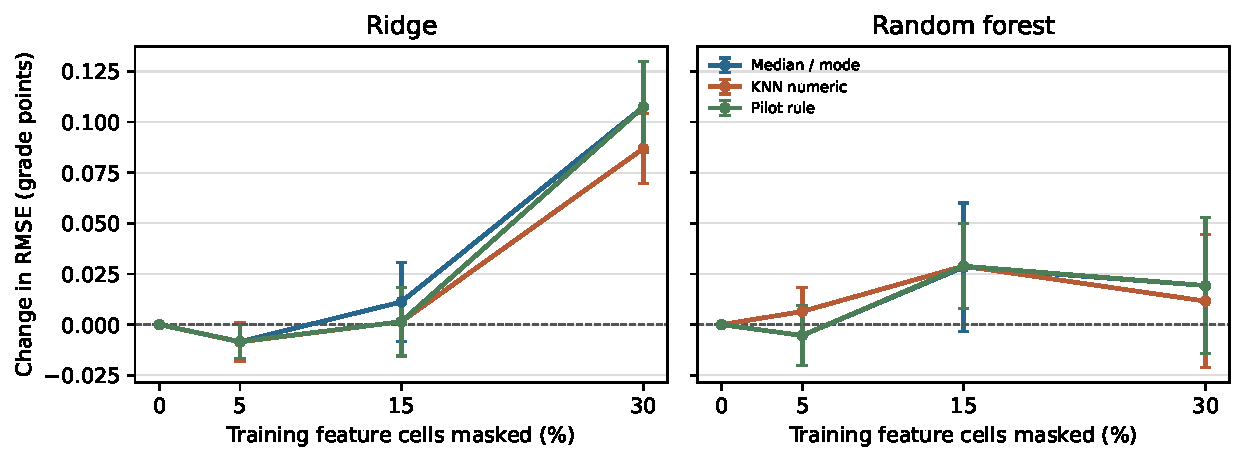
\includegraphics[width=0.82\textwidth]{pilot_rmse_delta.pdf}
\caption{Preliminary pilot: change in held-out RMSE relative to each split's uncorrupted median/mode result. Points are means over five splits and bars are standard errors across those splits. Only random training-feature missingness is tested; negative values at 5\% are sampling variation, not evidence that corruption helps.}\label{fig:pilot}
\end{figure*}

Table~\ref{tab:pilot} and Fig.~\ref{fig:pilot} show no meaningful advantage for the provisional rule. At 15\% masking the rule's mean difference from fixed median/mode is about $-0.010$ grade points for Ridge and approximately zero for the forest. At 30\% it returns to median/mode while KNN has lower mean RMSE in this one dataset. These small paired differences should not be read as a discovery. The apparent improvement at 5\% versus the uncorrupted mean is possible because the model and finite split vary; a corruption rate does not force monotonic degradation in every empirical run. The forest is comparatively stable here, but no claim about all tree models follows.

The pilot leaves several important threats unresolved. The mirror must be matched to the original data; the chosen policy thresholds were illustrative; one dataset provides no external validity; missingness is only MCAR-like; no numeric extremes were injected; and the neural comparison has not run. Consequently H2 remains untested as a general hypothesis. The next recorded experiment will freeze a revised policy before evaluating multiple datasets and will present the resulting per-dataset effects in this section. The final manuscript will replace this working-draft subsection with the completed analysis while preserving the pilot as supplementary context if useful.

\section{Conclusion}
DataSentry AI is framed as a controlled study of when cleaning choices improve tabular prediction, with an application to make the analysis inspectable. Prior research already establishes data-quality assessment, automated repair, and adaptive imputation. The specific paper question concerns whether a small transparent rule is worth using compared with fixed preprocessing under a leak-safe, paired benchmark. The measured student-data pilot does not support a meaningful benefit for its provisional rule. Broader experiments and a neural comparison are required before the paper can answer the central question. The final report will include negative outcomes, runtime, and limitations alongside any gains.

\bibliographystyle{IEEEtran}
\bibliography{references}
\end{document}
